\documentclass[Bachelorarbeit.tex]{subfiles}
\begin{document}

\newpage
\section{Sparse Lucas Kanade Optical Flow for Eye Movement Detection}
\label{Sparse Lucas Kanade Optical Flow}
%- to detect movement problem specific, good keypoints and parameters have to be found
%- no ground truth, hard to come by + no use, since we only detect movement and not classify
\todo{gesamtkonzept, keypoint detektoren}
In the following sections a method to search for the best setup for eye-movement analysis is carved out. These setups consisting of preprocessing, key point detection and Lucas-Kanade optical flow. Firstly, these setups are explained. Secondly, in \autoref{detectors}, key point detection in general is presented and the algorithms used in this work are explained in further detail. Thirdly, in \autoref{setup}, the structure for evaluation of these setups are defined. Lastly, the testing is presented in general on the scripts being used.\\
The sparse version of Lucas' and Kanade's method calculates the optical flow on a set of key points in the image.  
%A large amount of key point detection algorithms exist, an overview is given in \autoref{lk} \todo{an anfang}. 
Before the actual detection, preprocessing takes place to improve findings of key point detectors by removal of noise. The located key points found in the first frame function as input for optical flow. Based on the Lucas-Kanade method, the locations of these points are estimated on the next frame. If it is possible, the optical flow method can use the locations as new input for the next frame, repetitively. To calculate new locations of key points is called tracking in this thesis. The tracking of a point stops, if the Lucas-Kanade method can not estimate the new location of a point in the next frame. Furthermore, every 10 frames, additional key points are detected, with exactly the same method as in the first frame. To reduce false findings of the optical flow algorithm, a backwards check is implemented: The locations being estimated by the forward step serve as input for the estimation of original locations. If the estimation of the original location differ from the original location by more than 1 pixel, the tracking for this key point stops.

\subsection{Keypoint Detection}
\label{detectors}
A comparison of key point detectors and feature descriptors was done by \cite{gauglitz2011evaluation} for visual tracking. It includes six interest point detection algorithms, chosen because of their frequent use and previous tests. Based on their evaluation, three were chosen  for this thesis.
\subsubsection{Shi-Tomasi}
The key point detector developed by Shi and Tomasi yields corners. It can be viewed as a variation of the Harris corner detector \citep{harris1988combined}. \cite{shi1993good} developed it by analyzing which key points are good for tracking. In general, the neighborhood is viewed and the change in intensity is calculated with help of a structure tensor, which comprises this information in form of a symmetric 2 x 2 matrix:
\\
\\
	$M(x,y) =$
\begin{equation}
	\begin{bmatrix}
	\sum\limits_{u,v}w_{u,v}\cdot\left[I_x(x+u,y+v)\right]^2 & \sum\limits_{u,v}w_{u,v}\cdot I_x(x+u,y+v) I_y(x+u,y+v)~ \\
	~\sum\limits_{u,v}w_{u,v}\cdot I_x(x+u,y+v) I_y(x+u,y+v) & \sum\limits_{u,v}w_{u,v}\cdot\left[I_x(x+u,y+y)\right]^2
	\end{bmatrix}
\end{equation}
Where $M(x,y)$ is the structure tensor at location (x,y) in the image I, $I_x$ and $I_y$ denote derivatives of the image in x and y location, respectively. $w_{u,v}$ is a window and Gaussian weighting function, so the summations take place over the neighborhood of I(x,y). Based on the eigenvalues $\lambda_1$ and $\lambda_2$ of M, the image patch can be classified as uniform (both eigenvalues small), edge ($\lambda_1 small and \lambda_2 large, or vice versa$) or a corner (both values large.) Corners localized by this algorithm yield supposedly good features to track \citep[p. 3]{shi1993good}.
	
	
	
\subsubsection{Difference of Gaussian}
Difference of Gaussian (DoG), the key point detection algorithm used in Scale Invariant Feature Transform (SIFT) \cite{lowe2004distinctive}. This Blob detector extracts key points which are invariant to scale, an image is convolved with Gaussian kernels, having differing standard variations leading to various blurred versions of it. These are also called octave layers, with octaves being down-sampled versions of the input image, in this case, by taking every second pixel in each row and column. The process of convolution with Gaussian kernels is repeated on these octaves. Next, differences of Gaussians are achieved, by subtracting each octave layer from the next higher layer. Candidates for key points are those pixels, which yield local maxima compared to the 8 neighbors in its own difference of Gaussian and the 18 in the ones above and below it. In further analysis, candidates with low contrast and points along an edge are discarded, with an approach similar to corner detection \citep[pp. 94-98]{lowe2004distinctive}. 
\begin{center}
	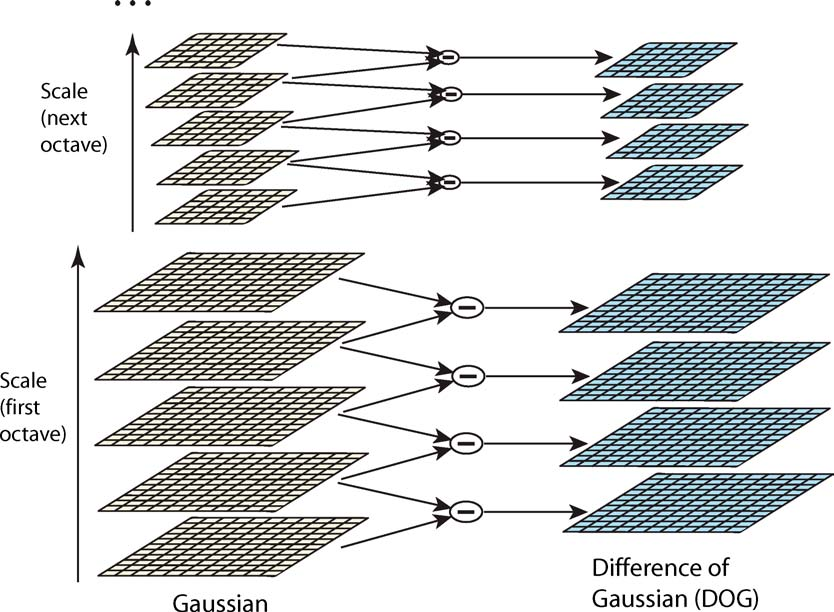
\includegraphics[width=0.7\linewidth]{Images/dog}
	\captionof{figure}{Difference of Gaussians is achieved by repeated convolution of the input image with Gaussian kernels and subsampling. Then, the octave layers are subtracted from each other.}
	\label{dog}
\end{center}
\begin{center}
	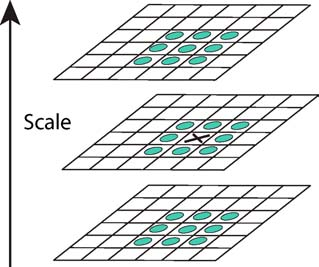
\includegraphics[width=0.4\linewidth]{Images/dog2}
\captionof{figure}{Candidates for key points are local extrema in comparison to their neighbors in the same, and neighboring octave layers.}
\end{center}
	
	%To obtain scale-invariant features, this process is repeated on down-sampled versions of the image and points of highest difference are selected on the appropriate scale. Key points are selected from extrema in subtractions of these versions, approximating the Laplacian.
	
\subsubsection{Fast Hessian}
Another Blob detector, the fast Hessian detector, was proposed by \cite{bay2006surf} for Speeded Up Robust Features (SURF), which was developed to enhance SIFT. Fast Hessian detects key points by approximation of the Hessian matrix, which is obtainable by convolution of the image with a Gaussian second-order derivatives. Since this is very costly, the convolution is approximated by simple box filters, which can be computed in constant time using the integral image \citep{viola2001rapid}. The scale-invariance is achieved by upscaling these filters and key points are chosen based on the highest determinant of the resulting, (fast) approximated, Hessian matrices in their corresponding scale. Similar to the difference of Gaussian approach, candidates of low contrast are rejected\citep{bay2006surf}.
\begin{center}
	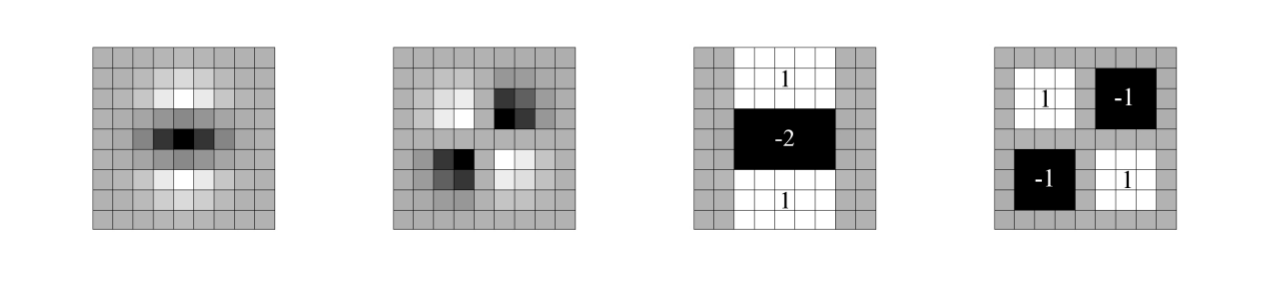
\includegraphics[width=0.7\linewidth]{Images/fhess1}
	\captionof{figure}{Second order Gaussian derivatives (left) are approximated as box filters (right) to receive an approximation of the Hessian matrix.}
\end{center}

\begin{center}
	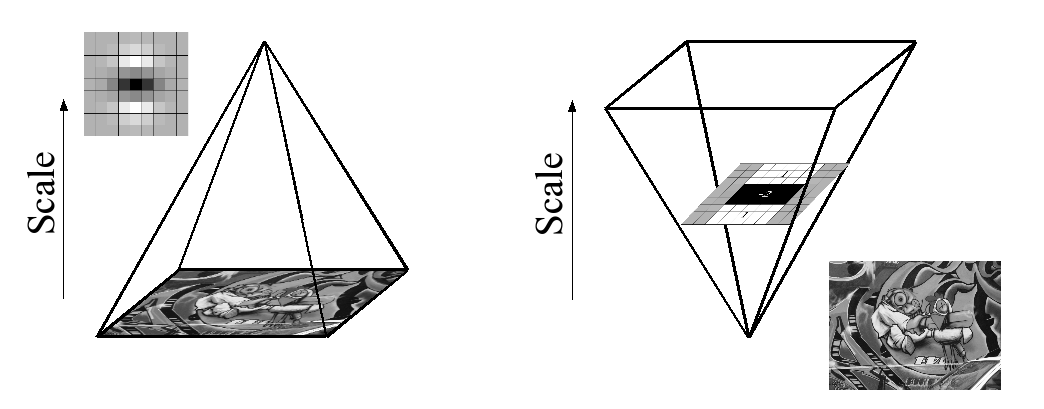
\includegraphics[width=0.7\linewidth]{Images/fhess2}
	\captionof{figure}{As opposed to the upscaling being done in key point detection with the difference of Gaussian approach (left), the image is not supsambled, but the box-filter is upscaled to include different scales.}
\end{center}

\subsection{Setup for Evaluation}
\label{setup}
In the following subsections, a setup to evaluate three methods to detect key points in eye-videos which can be tracked by the method of Lucas and Kanade. In the beginning, the dataset is explained, followed by qualitative measures to evaluate different setups to calculate optical flow with the Lucas-Kanade method, each including preprocessing of the data and key point detection. 
\todo{noch mehr intro}
\subsubsection{Dataset}
\label{dataset}
The data was acquired by filming a subject solving small tasks in virtual reality. Two cameras are located in the virtual reality glasses and pointed at the subject's left and right eye. Three different sets of videos exist. 10 subjects were filmed doing the newest version of the test, with an average video length of 5 minutes. The frame-rate corresponds to 120 Hz and the videos have a resolution of 640 x 320 pixel. 1 subject was recorded doing the same test, but at a frame-rate of 200 Hz and a resolution of 192 x 192 pixel. 8 subjects were recorded doing an older version of the test in virtual reality, which takes about 3 minutes, also at a framerate of 120 Hz and a resolution of 640 x 320 pixel. This dataset was annotated with timestamps of blinks. Examples for each dataset can be seen in \autoref{data_figure}. Even though the cameras are mounted to the subject's head, videos contain not only eyes, and not always every part of the eye. As seen in \autoref{data_figure}b), both canthi, the corners of eyes where the eyelids meet, are not visible in every video. Furthermore, unmoving, strong structures can be viewed in \autoref{data_figure}a) in the upper right corner. Beside this and noise in the recordings, another disruption of videos is visible. One infrared light can be seen turning on and off, leading to a so-called flicker in large parts of the images, as can be seen in \autoref{flicker_figure}. 
Even if it is not a very large dataset, it enables a lot of research with a wide variation of data.

\begin{center}
	
\begin{minipage}{0.48\linewidth}
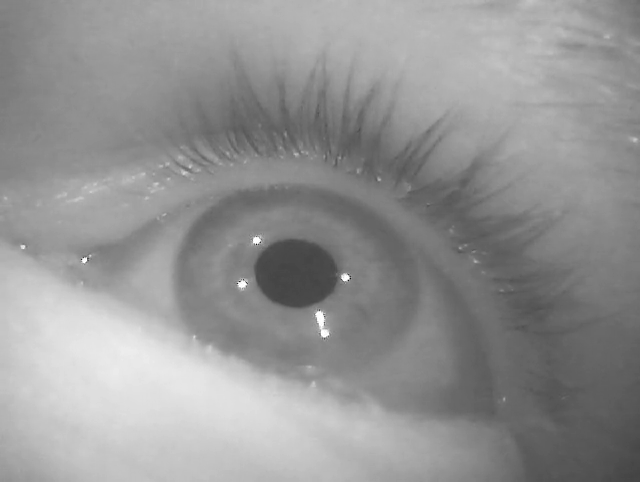
\includegraphics[width=\linewidth]{Images/no_blink_snap.png}
\captionof*{figure}{a)}

\end{minipage}
\begin{minipage}{0.48\linewidth}
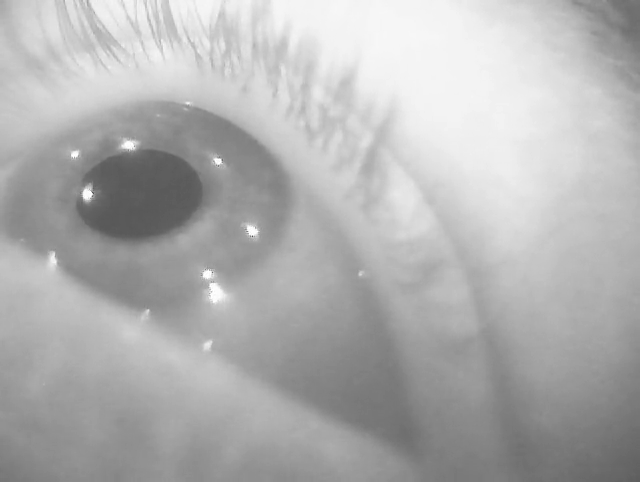
\includegraphics[width=\linewidth]{Images/part_missing.png}
\captionof*{figure}{b)}
\end{minipage}
\end{center}
\begin{center}
\begin{minipage}{0.48\linewidth}
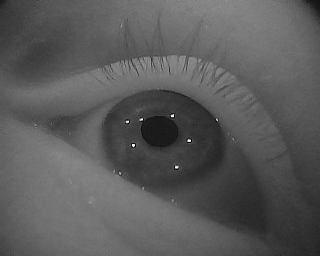
\includegraphics[width=\linewidth]{Images/blink_snap.png}
\captionof*{figure}{c)}
\end{minipage}
\begin{minipage}{0.48\linewidth}
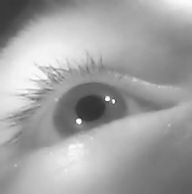
\includegraphics[width=\linewidth]{Images/200hz_snap.png}
\captionof*{figure}{d)}
\end{minipage}
\captionof{figure}{Variations of data: \textbf{a)} and \textbf{b)} 640 x 320 @ 120 fps. \textbf{c)} 320 x 240 @ 120 frames and \textbf{d)} 192 x 192 @ 200 fps. Rotation and camera angle are not identical, e.g. in \textbf{b)} only one canthi is part of the image. }
\label{data_figure}
\end{center}
\begin{center}
\begin{minipage}{0.48\linewidth}
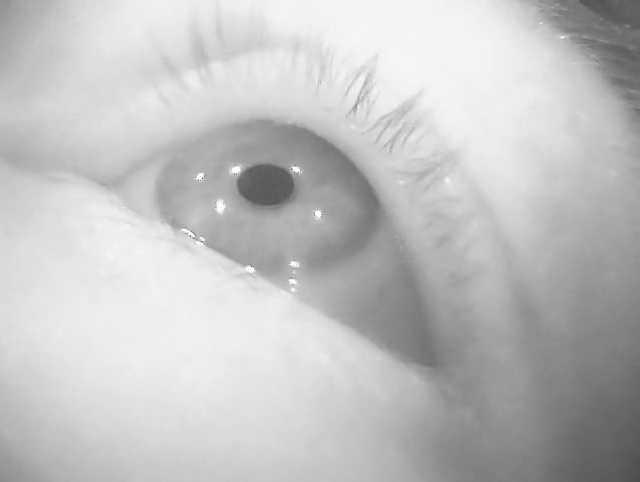
\includegraphics[width=\linewidth]{Images/flicker_1.png}
\captionof*{figure}{a)}
\end{minipage}
\begin{minipage}{0.48\linewidth}
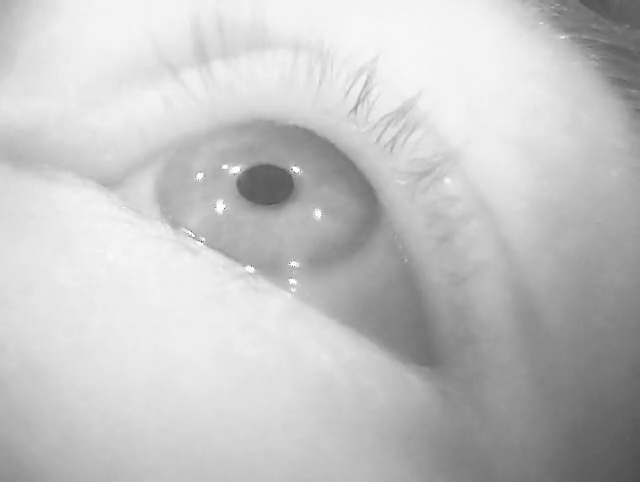
\includegraphics[width=\linewidth]{Images/flicker_2.png}
\captionof*{figure}{b)}
\end{minipage}
\captionof{figure}{Flicker}{Flashing of light leads to a 'flicker'. Consecutive frames vary in brightness.}
\label{flicker_figure}

\end{center}

%- headmounted eye tracker, nearly only eye in image
%- fps, resolution, length
\subsubsection{Measures}
In the following section, the qualitative measures taken to validate the setups for calculating optical flow are compared. In this thesis, qualitative measures are those, which do not rely on ground truth, e.g., it is not determined, whether the optical flow of the eye being calculated is the correct one, measured in another way or via human validation. As opposed to such quantitative measures, qualitative ones can be helpful to compare these methods in relation to each other.

\subsubsection*{Quantity and Runtime}
\label{quan}
To have a basic measure to compare detection algorithms, found key points are counted. Additionally, parts in the video, in which no key points can be found or have been tracked are noted. To have this basic measure is important, because a very small number of key points leads to small computational effort for the optical flow method, but one can argue that a small change in the setting (lighting, shift of camera etc.) leads to problems for the optical flow algorithm to track these points. This is also true, if a lot of points are being tracked, but in that case, the chance is higher to have additionally a few trackable points. On the other hand, a large number of key points is computationally suboptimal. Also, it is most often paired with a short lifespan of key points and therefore not desirable. Accordingly, a medium number of key points is desired. \\
Another simple measure is the runtime of the overall algorithm. Even though the application is not supposed to be in real time, a faster algorithm which yield the same results as another is superior to it.


%- basic
%- important for computational time
%- robustness
%- compare other measures

\subsubsection*{Lifespan}
\label{lifespan}
\begin{center}
	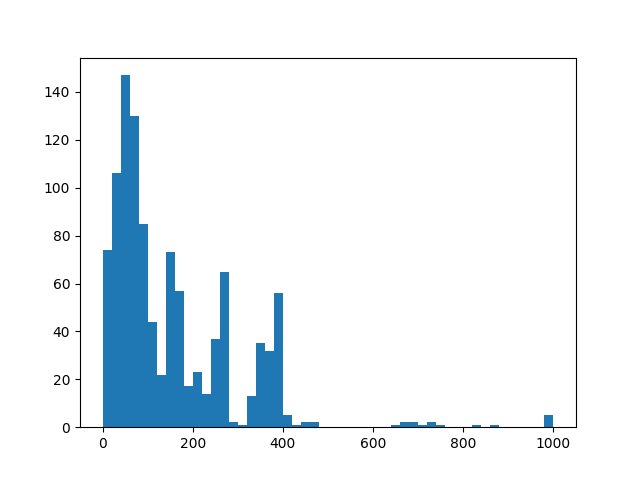
\includegraphics[width=0.7\linewidth]{Images/hist_proto}
	
	\captionof{figure}{Histogram of quantity of keypoints being tracked over time in frames }\todo{beschriftung!!}
	\label{hist_im}
\end{center}
A second measure for comparison is how long optical flow can track the found key points, the so-called lifespan. In particular, it supplies the sum of how often the Lucas-Kanade optical flow can calculate the location of a point in the following frame. This can easily be counted and is essential for comparison. First, the average lifespan over all videos is calculated and the best few are selected. In further analysis, a histogram is helpful, see \autoref{hist_im}. The data is visible for a part of a video comprising 1000 frames and using the Shi-Tomasi corner detector. The data is rounded to decades. A peak is visible at a lifespan of ~80 frames with over 140 tracks. A lot of

\todo{aktuelles histogram, beschreibung dafür, infos: params, avg. lifespan, wie viele keypoints etc}




- how long can optical flow track?
- important to see with distribution

\subsubsection*{Spatial Distribution of Key Points}
\label{dist}
\begin{center}
	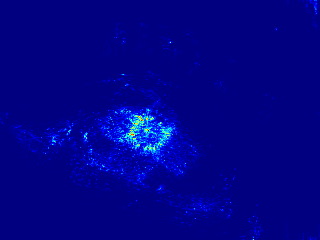
\includegraphics[width=0.5\linewidth]{Images/heatmap_proto}
	\captionof{figure}{Heatmap of duration of tracking in image plane.}
	\label{heatmap}
\end{center}
A third qualitative measure for the detection algorithms is where key points are located. Included is the location of points that are found by a detection algorithm, but also the locations which have been estimated by the optical flow algorithm. Figure 4 shows a heatmap which presents this information. By comparison with the actual image in the video it is possible to see if the locations are semantically relevant. Distribution over the whole image are desired. Especially so over moving parts, as this is information directly valuable for the task at hand, being motion detection. But also key points tracked at generally unmoving parts are important because if movement is measured there, a disruption of world parameters is likely, e.g. a change in the location of the camera or lighting conditions. 
\\It is important to carefully examine these measures with respect to each other. A very high lifespan is a generally desirable result, but if there are just a few key points found, which are all located in unmoving parts of the video it is still not a good outcome. The same can be said about a well distribution of key points over the images with a very small average lifespan, since it signifies that key points can not be tracked well with the optical flow method.

%- where are the keypoints located?
%- semantically relevant?
%- good: distributed over whole image
%- even without movement, explanation for moving of camera!

\subsection{Preprocessing}
\label{preprocessing}
To improve the accuracy of movement detection it is of importance to remove irregularities from the data. The techniques to process the videos before detecting key point alter the findings significantly and their parameters are therefore a part of testing. The frames are filtered with Gaussian or median kernels and resized via interpolation. This reduces noise and also possibly destroys larger structures seen in the image, depending on the kernel size. Destruction of those could lead to a better measurment, because they are unmoving.\todo{entscheide, ob du die zerstören willst oder nicht} The smaller sizes and (median-) filtering leads to a larger difference of pixels beside each other and therefore more key points to find \todo{ref}
\todo{bilder einfügen}
%When watching the videos, a hardware circumstance is visible: one of the infrared lamps of the eyetracker is turning on and off, leading to a flicker in some videos (\autoref{flicker_figure}).
To test if the flicker, as explained in \autoref{dataset}, has significant impact on the performance of the tested motion analysis, a procedure to remove this flicker is applied. Midway equalization, as shown by \cite{delon2004midway} takes the histogram of gray values from two or more consecutive frames and calculates an equalized version, changing the values of the single frames.  

 
%- processing steps have to be taken
%- deflickering
%- resizing und filtering: testen, wie gut mit mweasures, detectors, optical flow

\subsection{Testing}
\label{testing}

In this section, implementations to gain information to measure, as explained in \autoref{setup} are presented. The machine is working with Python 3.7.4 and OpenCV 4.1.1. To be tested is the following: parameters for detection algorithms, parameters for Lucas-Kanade optical flow, and preprocessing. Because the computational load would explode by testing all combinations at once, not every configuration of parameters is going to be tested. \todo{vlt eine rechnung?} Rather, three steps are applied: First, detector parameters are tested with a fixed framework of optical flow and preprocessing steps. Second, the framework is set with fixed parameters for the detection algorithms proven to be best and fixed preprocessing and optical flow is tested with these. In a third step, preprocessing is tested with fixed optical flow and key point detection. Afterwards, key point detectors will be tested again to validate the results. What follows is a listing of parameters with a short explanation.

\subsubsection{Shi-Tomasi Corner Detector}
The Shi-Tomasi detector is implemented in the used version of OpenCV in use as cv2.goodfeaturestotrack() and users can change it with the following parameters \citep{itseez2019theopencv}:
\begin{itemize}
	\item maxCorners. This is the maximum number of returned key points.
	\item qualityLevel. A number between 0 and 1, which determines how strong the measure in a point has to be. All candidates are compared with the best one found. To be considered a key point, the corner measure has to be at least 90 percent as good as the best one found, if the qualityLevel parameter is set to a value of 0.9.
	\item minDistance. The minimal Euclidian distance between points to be considered a key point.
	\item blockSize. Size of the neighborhood included by the structure tensor.
\end{itemize}

\subsubsection{Fast Hessian}
The Fast Hessian detector is bound to SURF in OpenCV. As only the detection of key points is needed, a SURF object is created with  and key points are detected with cv2.xfeatures2d.SURF\_create().detect() \citep{itseez2019theopencv}. The following parameters were tested:
\begin{itemize}
	\item hessianThreshold. The main part of key point detection with this detector is the threshold for the determinant of the approximated Hessian matrix.
	\item nOctaves. How often the filter is upscaled to yield different scales.
	\item nOctaveLayers. How often the filter is upscaled at each octave.
\end{itemize}


\subsubsection{Differences of Gaussian}
The Differences of Gaussian detector is bound to SIFT in OpenCV. Same as for SURF, only the keypoint detection is needed, it is evoked by calling cv2.xfeatures2d.SIFT.create().detect() \citep{itseez2019theopencv}. Parameters concerning keypioint detection are listed here:
\begin{itemize}
	\item nfeatures. The number of best key points to hold on to, ranked by local contrast.
	\item nOctaveLayers. The number of times the Gaussian convolution is applied to each octave with higher standard deviation to yield blurred versions of the octave. Returns difference of Gaussian by subtraction to the function. Differing standard deviations are calculated automatically by the resolution.
	\item Octaves. The number of times, the input image is downsampled.
	\item contrastThreshold. This threshold rejects key point candidates which have a low contrast.
	\item edgeThreshold. This threshold rejects key point candidates which are located on edges, and not corners.
	\item sigma. The standard deviation applied to the first octave of the input image. 

\end{itemize}


\subsubsection{Lucas Kanade optical flow}
The Lucas Kanade optical flow method is implemented in the OpenCV library as cv2.calcOpticalFlowPyrLK() and uses the following parameters:
\begin{itemize}
	\item winSize. The window in which the algorithm searches in the new frame for the new location of the key points, on all levels.
	\item maxLevel. The maximum number of levels of reduction to use.
	\item criteria (cv.TERM\_CRITERIA\_EPS | cv.TERM\_CRITERIA\_COUNT) Specifies the criterion to stop the search algorithm, either by number of iterations (COUNT) and/or after the search window moves by less than epsilon (EPS).
\end{itemize}

\subsubsection{Preprocessing}
\todo{wie mach ich das mit abkürzung, lk opt flow?}
To test the improvement of precision by detection and tracking of key points by altering the preprocessing steps, the following steps are taken into account:
\begin{itemize}
	\item Downsampling by bilinear interpolation, as is used by cv2.resize()
	\item Noise-removal: Gaussian kernels, as well as median filtering is being used. The latter mainly to destruct medium-sized, unmoving structures (i.e. eyebrows) to focus key points on moving, large objects (pupil, iris, eye-lids).
	\item Deflickering. Keypoint detectors are tested on the videos with removed global flicker, to improve the optical flow algorithm. 
\end{itemize}


- explain scripts: testing.py, gfeattesting.py etc
cycle: testing detectors with fixed values for lkparams und preprocessing
dann fixed detectors, lk params
dann fixed detectors, preprocessing
dann noch einmal keypoint detectors


\FloatBarrier
\end{document}